% !TeX spellcheck = ca
\documentclass{article}
\usepackage[utf8]{inputenc}
\usepackage{graphicx}
\usepackage{tikz}
\usepackage{listings}
\usepackage{float}
\usepackage{amsmath}
\usetikzlibrary{positioning,fit,calc,arrows.meta, shapes}
\graphicspath{ {images/} }

%Tot això hauria d'anar en un pkg, però no sé com és fa

\newcommand*{\assignatura}[1]{\gdef\1assignatura{#1}}
\newcommand*{\grup}[1]{\gdef\3grup{#1}}
\newcommand*{\professorat}[1]{\gdef\4professorat{#1}}
\renewcommand{\title}[1]{\gdef\5title{#1}}
\renewcommand{\author}[1]{\gdef\6author{#1}}
\renewcommand{\date}[1]{\gdef\7date{#1}}
\renewcommand{\contentsname}{Índex}
\renewcommand{\maketitle}{ %fa el maketitle de nou
	\begin{titlepage}
		\raggedright{UNIVERSITAT DE LLEIDA \\
			Escola Politècnica Superior \\
			Grau en Enginyeria Informàtica\\
			\1assignatura\\}
		\vspace{5cm}
		\centering\huge{\5title \\}
		\vspace{3cm}
		\large{\6author} \\
		\normalsize{\3grup}
		\vfill
		Professorat : \4professorat \\
		Data : \7date
\end{titlepage}}
%Emplenar a partir d'aquí per a fer el títol : no se com es fa el package
%S'han de renombrar totes, inclús date, si un camp es deixa en blanc no apareix

\renewcommand{\figurename}{Figura}
\renewcommand{\tablename}{Taula}
\title{Práctica 1}
\author{Quim Picó Mora, Ian Palacín Aliana}
\date{18 d'Octubre 2019}
\assignatura{Sistemes Concurrents i Paral·lels}
\professorat{F. Cores}
\grup{PraLab1}

%Comença el document
\begin{document}
	\maketitle
	\thispagestyle{empty}
	
	\newpage
	\pagenumbering{roman}
	\tableofcontents
	\newpage
	\pagenumbering{arabic}
	


% Petita estimació de si el sistema serà útil per l’empresa i és factible de ser desenvolupat 
% sota les restriccions existents, a fi de determinar si es tira endavant, o bé val la pena invertir 
% en un estudi de viabilitat més profund i seriós
%TODO: @horno Fes aquesta part

%. Domini  (NO es demana)
%Glossari de termes del domini

\section{Introducción}

En este documento se compara la eficiencia en tiempo que supone ejecutar la aplicación calcArboles de forma concurrente respecto de forma sequencial. También se muestra a continuación la mejora en tiempo que supone el paral·lelismo de hilos durante la ejecución del programa.
\\\\
Los datos que se utilizaran para hacer el estudio saldrán de ejecutar de forma sequencial y concurrente los mismos ejemplos, calculando así el tiempo en que tarda en realizarse cada una de las ejecuciones. Este tiempo será el que luego se usará para comparar y sacar conclusiones.\\
De mismo modo se ejecutará varias veces el programa con distinto número de hilos de ejecución y se procederá a la comparación de los resultados.


\section{Concurrente vs Sequencial}

\begin{figure}[hbt!]
  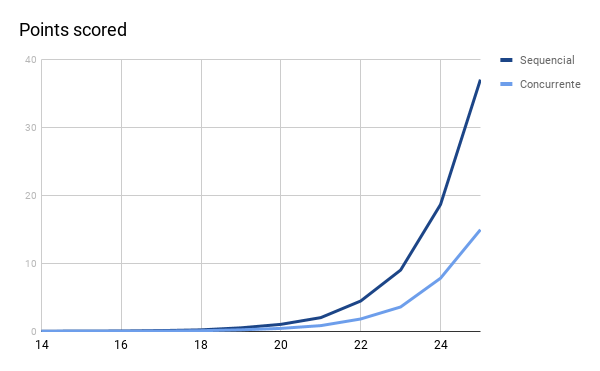
\includegraphics[width=\linewidth]{concuvsseq.png}
  \caption{Concurrente vs Sequencial}
  \label{fig:convsseq}
\end{figure}
\newpage
%escriure a partir d'aquí

\section{Diferencias entre multiples hilos}
\begin{figure}[hbt!]
  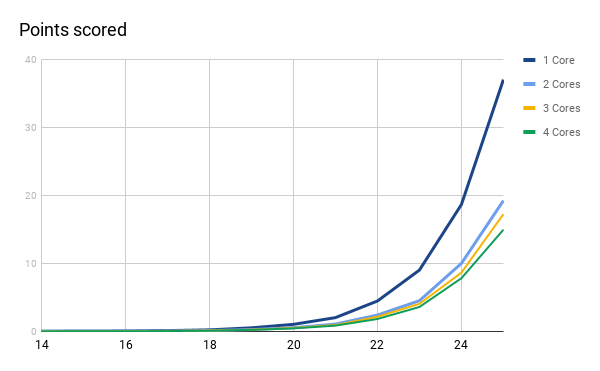
\includegraphics[width=\linewidth]{multihilo.png}
  \caption{Ejecucion con múltiples hilos}
  \label{fig:multhilos}
\end{figure}

\end{document}

